% !TeX encoding = UTF-8
% !TeX spellcheck = pl_PL

\def\filename{Rozdział 2}

\chapter{Prognoza wyborów w~ujęciu teoretycznym}

\section{Podział na okręgi wyborcze}

Świat polityki w~Polsce cechuje się dość dużą niestabilnością. Pojawianie się nowych ugrupowań, upadki starych powodują, że wszelkie formy przewidzenia i~prognozowania sytuacji politycznej za ileś lat skazane są na porażkę. Z tego powodu opisywana w~tej pracy symulacja wyników musi posiadać pewne założenia. Pierwszym z~nich jest symulowanie wyników tak jakby nowa ordynacja wyborcza już obowiązywała w~dniu wyborów do Sejmu RP w~2019 roku. Należy też pamiętać, że strategie partii politycznych są ustalane według panujących zasad ordynacji wyborczych. Ordynacja ma wpływ na liczbę i~kolejność osób na listach, dobór partii koalicyjnych, czy nawet hasła i~programy głoszone przez kandydatów.

Kolejnym założeniem jest charakter wyborów. Na potrzeby pracy założono, że wprowadzono system obowiązujący w~Wielkiej Brytanii. To znaczy, że mandat poselski w~danym okręgu zdobywa ta osoba, która po prostu zdobędzie najwięcej głosów. Nie zakładamy przeprowadzania drugiej tury, systemu głosów przechodnich itp. 

Ponieważ nowa ordynacja wymaga stworzenia zupełnie nowego podziału terytorium Polski na nowe okręgi wyborcze, w~znacznie większej niż dotychczasowej liczbie, wykorzystano już gotowy projekt podziału przygotowany przez Fundację im. J. Madisona, której celem jest promowanie wprowadzenia nowej ordynacji wyborczej. Fundacja w~ramach swojej działalności przygotowała projekt ustawy zmieniającej aktualny kodeks wyborczy wraz z~nowym podziałem okręgów wyborczych. Podział przygotowany przez Fundację im. Madisona zakłada, że okręgi wyborcze w~swoich granicach nie obejmuje terenów więcej niż jednego województwa, gminy nie powinny być dzielone pomiędzy różne okręgi, a~liczba wyborców w~okręgach powinna być zbliżona. Duże miasta są dzielone na okręgi według już istniejących podziałów na obwody wyborcze. Zarezerwowano również jeden okręg dla obywateli polskich poza granicami kraju. Numeracja okręgów z~przypisanymi województwami jest przedstawiona poniżej:

\begin{table}[h!]
\caption{Wykaz okręgów wyborczych}
\centering
\begin{tabular}{|l|c|l|}
\hline
\multicolumn{1}{|c|}{\textbf{Nr okręgu}} & \textbf{Liczba} & \multicolumn{1}{c|}{\textbf{Województwo}} \\ \hline
1-35                                     & (35 okręgów)    &  dolnośląskie                         \\ \hline
36-60                                    & (25 okręgów)    &  kujawsko-pomorskie                   \\ \hline
61-86                                    & (26 okręgów)    &  lubelskie                            \\ \hline
87-98                                    & (12 okręgów)    &  lubuskie                             \\ \hline
99-129                                   & (31 okręgów)    &  łódzkie                              \\ \hline
130-169                                  & (40 okręgów)    &  małopolskie                          \\ \hline
170-232                                  & (63 okręgi)     &  mazowieckie                          \\ \hline
233                                      & (1 okręg)       & zagranica                                 \\ \hline
234-245                                  & (12 okręgów)    &  opolskie                             \\ \hline
246-270                                  & (25 okręgów)    &  podkarpackie                         \\ \hline
271-284                                  & (14 okręgów)    &  podlaskie                            \\ \hline
285-311                                  & (27 okręgów)    &  pomorskie                            \\ \hline
312-367                                  & (56 okręgów)    &  śląskie                              \\ \hline
368-382                                  & (15 okręgów)    &  świętokrzyskie                       \\ \hline
383-399                                  & (17 okręgów)    &  warmińsko-mazurskie                  \\ \hline
400-440                                  & (41 okręgów)    &  wielkopolskie                        \\ \hline
441-460                                  & (20 okręgów)    &  zachodniopomorskie                   \\ \hline
\end{tabular}
\caption*{Źródło: \url{madison.org.pl/kodeks-wyborczy-jow/}}
\end{table}

Wadą projektu ustawy Fundacji Madisona jest jej niedoskonałość. Istnieje pewna dysproporcja w~liczbie wyborców w~każdym z~okręgu. Średnia wielkość okręgu wynosi 65800 uprawnionych do głosowania i~takiej liczbie powinna być bliska liczba uprawnionych w~każdym z~okręgów. Jednak odchylenie standardowe wynosi aż 15172, co oznacza że to założenie jest niespełnione. Należy od razu zwrócić uwagę, że największy z~okręgów ze względu na swoją nadzwyczajną specyfikę ma aż 349122 wyborców i~jest to okręg nr 233, obejmujący całą zagranicę. Ze względu na bardzo niską frekwencję wśród Polonii zagranicznej tak duża liczba uprawnionych nie ma faktycznego znaczenia \cite{Wilczyński}.

Najmniejszy okręg na terenie kraju to okręg nr 205 - Lipsko i~Zwoleń - 36 723 wyborców, obejmujący obszary wiejskie, a~największy okręg nr 218 - Warszawa Bielany - 104 178 wyborców. Taka dysproporcja może być spowodowana chęcią niedzielenia pojedynczych gmin oraz dzielnic miasta przez autorów projektu ustawy. Ze względu na apolityczny charakter Fundacji można mieć pewność, że opisane dysproporcje nie mają charakteru politycznego i~nie faworyzują celowo którejś z~formacji politycznych.

Posiadając opisane powyżej założenia można określić w~jaki sposób mogą zmienić się wyniki wyborów.

\section{Patologie związane z~podziałem państwa na okręgi wyborcze}
W wielu państwach, w~których obowiązuje JOW dochodzi z~biegiem czasu do coraz większych patologii. Co do zasady kształty okręgów wyborczych oraz co za tym idzie liczba wyborców w~nich mieszkająca powinny być ustalone sprawiedliwe, aby nie było możliwości, że jeden głos jednego wyborcy będzie mniej warty od innego.

\subsection{Nierówność okręgów}
Przykładowo Wielka Brytania, w~której obowiązujący system trwa już od wielu dziesięcioleci, różnica w~liczbie mieszkańców okręgów stała się bardzo znacząca. Największy okręg (ang. \textit{constituency}) Isle of Wight, obejmujący swoim obszarem całą wyspę Wight w~południowej Anglii, w~2019 roku miał aż 113 021 wyborców. Jednak z~powodów geograficznych i~kulturowych podział wyspy i~zmiany terytorialne okręgu stanowią pewne wyzwanie. Najmniejszy okręg to Na h-Eileanan an Iar położony na archipelagu Hebryd Zewnętrznych w~północno-zachodniej Szkocji z~21 106 wyborcami. W~tym przypadku odizolowanie geograficzne, duża odrębność kulturowa i~przywiązanie mieszkańców do swojego regionu jeszcze bardziej utrudnia zmiany w~graniach okręgu. Oznacza to, że siła głosu mieszkańca Hebryd Zewnętrznych jest ponad pięciokrotnie większa od mieszkańca wyspy Wight \cite{Baston}.

\subsection{Gerrymandering}
Innym przykładem patologii jest zjawisko Gerrymanderingu. Nazwa zjawiska pochodzi od połączenia słów \enquote{salamandra} oraz nazwiska gubernatora Massachusetts Elbridge'a Gerry'ego, który w~1812 roku utworzył w~swoim stanie dystrykt wyborczy w~kształcie właśnie podłużnej salamandry, aby zwiększyć szanse kandydatów z~partii demokratyczno-republikańskiej, nie patrząc na zależności kulturowe i~geograficzne swojego stanu. Gerrymandering jest typową manipulacją polityczną, która stała się bardzo popularna w~Stanach Zjednoczonych, zarówno wśród polityków demokratycznych jak i~republikańskich, którzy mają wpływ na kształt okręgów.

W celu zapobiegania tego typu manipulacjom od dawna proponuje się w~USA prawne wprowadzenie regulacji matematycznych. Jednak z~powodu dominacji dwóch partii - Republikańskiej i~Demokratycznej, których obu politycy stosują manipulację granicami, tego typu regulacje nie udają się wprowadzić.

Jednym z~matematycznych sposobów określenia czy podział na okręgi jest sprawiedliwy lub nie, jest wskaźnik EG (efficiency gap), który określa stosunek głosów zmarnowanych oddanych na dwie partie w~okręgu (przy uproszczonym założeniu, że tylko dwie biorą udział w~wyborach) \cite{Łeń}.
\begin{itemize}
    \item $D = {\delta_1, \delta_2, ..., \delta_s}$ - zbiór okręgów,
    \item $D^P \subset D $ - zbiór okręgów, w~których wygrała partia $P$,
    \item $V_i^P$ - liczba głosów zdobytych przez partię $P$ w~okręgu $\delta_i$,
    \item $V^P$ - całkowita liczba głosów oddanych na partię $P$,
    \item $V_i$ - liczba wszystkich głosów oddanych w~okręgu $\delta_i$,
    \item $V$ - liczba wszystkich głosów oddanych w~wyborach,
    \item $S_i^P$ - liczba miejsc zdobytych przez partię $P$ w~$i$-tym okręgu ($S_i^P \in {0, 1}$),
    \item $S^P$ - liczba wszystkich miejsc zdobytych przez partię $P$,
\end{itemize}

\begin{equation}
    v = \frac{V^A - V^B}{V}, \sigma = \frac{S^A-S^B}{S}
\end{equation}

\begin{itemize}
    \item $v$ - przewaga partii w~głosach,
    \item $\sigma$ - przewaga partii w~mandatach.
\end{itemize}
Głosami zmarnowanymi nazywamy głosy oddane na partię przegraną oraz te głosy na partię wygraną, które przekraczają pułap 50\%. Oznacza to, że zawsze 50\% głosów jest zmarnowane.
\begin{itemize}
    \item $W_i^P$ - liczba głosów zmarnowanych w~okręgu $\delta_i$ przez głosujących na partię $P$,
    \item $W^P$ - liczba zmarnowanych głosów we wszystkich okręgach,
    \item $EG$ - wskaźnik \textit{efficiency gap}.
\end{itemize}
\begin{equation}
    EG = \sum_{i=1}^{S}  \frac{W_i^A - W_i^B}{V} = \frac{W^A - W^B}{V}
\end{equation}

Przyjmuje, że gdy:
\begin{itemize}
    \item $EG > 0$ - niesprawiedliwość wobec partii $A$,
    \item $EG < 0$ - niesprawiedliwość wobec partii $B$,
    \item $EG \approx 0$ - obie partie straciły podobną liczbę głosów. Sytuacja jest uważana za sprawiedliwą. 
\end{itemize}

\newpage

W przypadku wyznaczania granic należałoby brać pod uwagę powyższy wskaźnik. Niestety nie jest on doskonały i~nie bierze pod uwagę wszystkich aspektów sprawiedliwości. Nie można założyć, że każdy okręg jest równy oraz, że w~każdym oddano taką samą liczbę głosów. Ponadto należy pamiętać o czynnikach geograficznych i~kulturowych w~określaniu granic okręgów. Niesprawiedliwość gerrymanderingu może jeszcze obrazować poniższa ilustracja \cite{Pierzgalski}.

\begin{figure}[H]
    \centering
    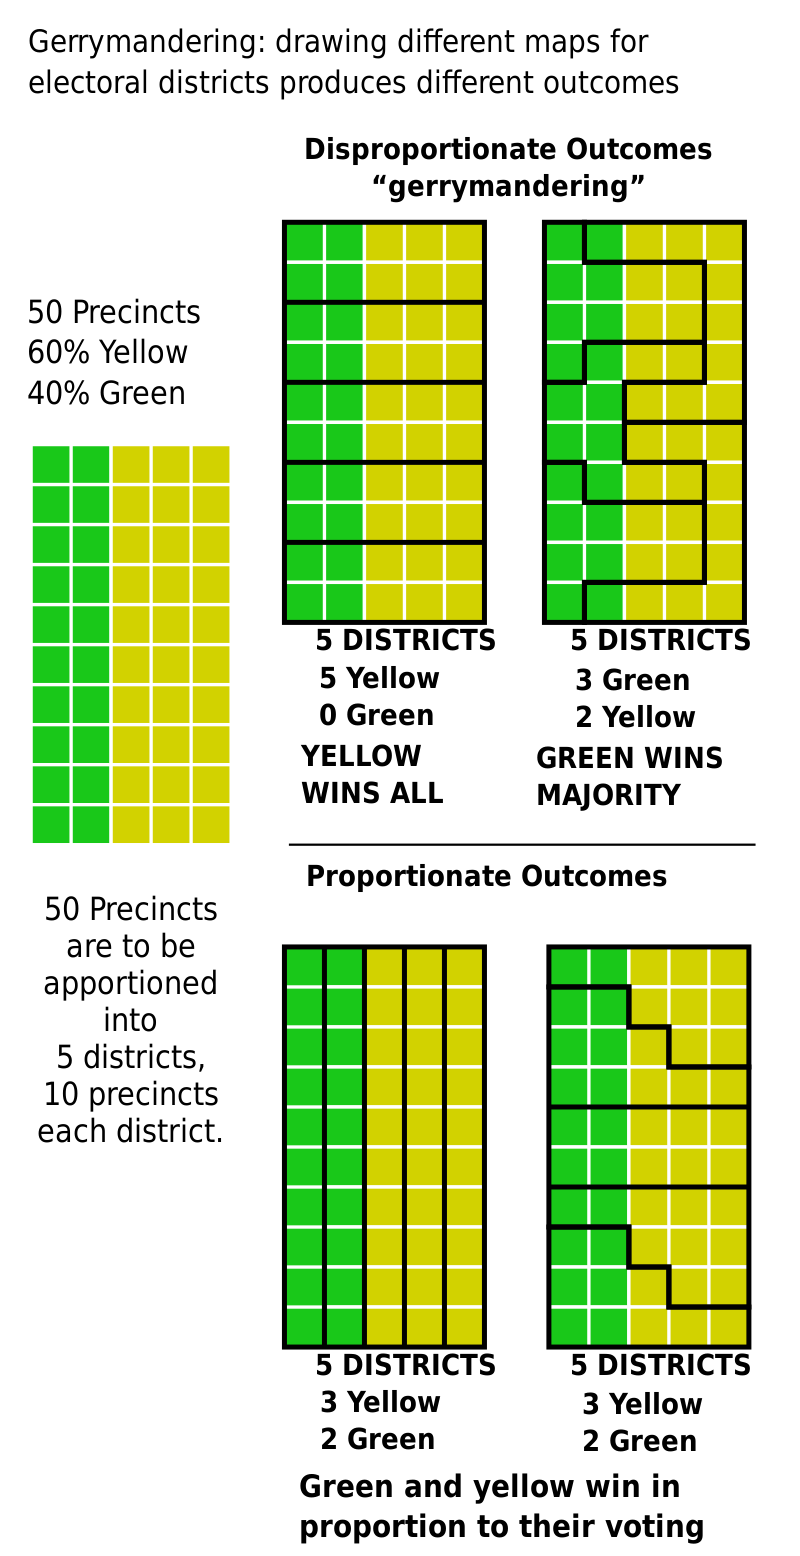
\includegraphics[width=0.5\textwidth]{rozdzial2/800px-DifferingApportionment.svg.png}
    \caption{Różne sposoby podziału na JOW}
    \caption*{Źródło: \url{https://commons.wikimedia.org/wiki/File:DifferingApportionment.svg}}
    \label{fig:my_label}
\end{figure}

\section{Zachowanie wyborców przy zmianie ordynacji wyborczej}

Kwestia zachowania wyborców jest bardzo trudna do przewidzenia. Wynika to z~tego, że zachowania ludzi są bardzo często nielogiczne. Ponadto liczne zmiany na scenie politycznej, powstawanie nowych partii, kompromitacje starych, łączenie się małych partii w~duże oraz podziały dużych jeszcze bardziej komplikują prowadzenie wszelkich poważnych prognoz nawet na 1 rok do przodu. 

Zmiana ordynacji wyborczej na jednomandatowe okręgi wyborcze zupełnie zmienia charakter wyborów. Do tej pory wyborca wybierając kandydata z~listy kierował się głównie tym do jakiej partii on należy oraz jaki program, jaki światopogląd ta partia prezentuje oraz jaki jest jej lider. Cechy pojedynczego kandydata były aspektem drugo- czy nawet trzeciorzędnym. W~JOW na pierwszy plan wychodzi kandydat z~małego okręgu. Co do zasady musiałby mieć zaufanie lokalnych mieszkańców, reprezentować nie tylko swoje poglądy, ale też interesy lokalnej społeczności. Jednak jak pokazuje doświadczenie krajów gdzie ten system już funkcjonuje i~tak kandydat, który nie ma poparcia jednej z~głównych partii politycznych nie ma szans na uzyskanie mandatu. W~Anglii są to Partia Pracy i~Partia Konserwatywna, w~USA Partia Republikańska i~Partia Demokratyczna. W~przypadku Polski głównymi obozami politycznymi jest Zjednoczona Prawica tworzona głównie przez Prawo i~Sprawiedliwość oraz obóz tzw. demokratycznej opozycji, który pomimo wielu różnic programowych i~światopoglądowych jest w~stanie współpracować tworząc wspólne listy oraz wystawiając wspólnych kandydatów jako opozycja wobec Zjednoczonej Prawicy. Tzw. demokratyczną opozycje tworzą Koalicja Obywatelska (głównie Platforma Obywatelska), partie lewicowe (SLD, Wiosna, Lewica Razem) oraz Polskie Stronnictwo Ludowe. Oczywiście tego typu podziały są bardzo zmienne i~zależą często wyłącznie od aktualnej sytuacji politycznej. Problem jest z~partią Konfederacja, która ze względu na swój wolnorynkowy program gospodarczy nie wpisuje się ani do obozu Zjednoczonej Prawicy ani ze względu na konserwatywny program światopoglądowy do partii opozycyjnych.
Na potrzeby pracy przeprowadzimy dwa scenariusze, różniące się zachowaniem wyborców.

\subsection{Scenariusz I}
W tym scenariuszu zakładamy, że wybory do Sejmu RP w~2019 roku zostały przeprowadzone z~zastosowaniem JOW, a~każdy wyborca zagłosował na kandydata tej partii, której listę w~rzeczywistości poparł. To znaczy, że uwzględniamy wszystkie partie bez względu na poziom ich poparcia.

\subsection{Scenariusz II}
Scenariusz II zakłada, że dochodzi do konsolidacji partii politycznych w~dwa duże bloki polityczne na wzór amerykańskich partii Demokratycznej i~Republikańskiej, a~wraz z~nimi przejęcie dotychczasowych wyborców. Zakładamy, że bloki będą dwa. Jeden reprezentujący prawicę, a~drugi lewicę, w~ich polskim rozumieniu.

W Polsce głównymi stronami osi sporu politycznego jest z~jednej strony Prawo i~Sprawiedliwość reprezentujący tak zwaną prawicę, pomimo swego dość interwencjonistycznego spojrzenia na gospodarkę, po drugiej stronie są partie bardziej liberalne światopoglądowo: Platforma Obywatelska oraz partie lewicowe. Problemem jest przypisanie wyborców innych partii niż PO i~PiS do nowych hipotetycznych bloków wyborczych.

Pomocą mogą być tutaj wybory na urząd Prezydenta RP, składające się z~dwóch tur głosowania. W~pierwszej turze wyborca może zagłosować na jednego z~wielu kandydatów (w 2020 roku było to 11 kandydatów). Do drugiej tury przechodzi już tylko dwóch kandydatów z~największą liczbą głosów, o ile było ich mniej niż 50\%. Wyborcy pozostałych kandydatów są niejako zmuszeni do zagłosowania na kandydata innej opcji. Dzięki temu można było przebadać w~jaki sposób rozdzielały się elektoraty pozostałych kandydatów. Zakładając, że wyborcy mniejszych partii zachowają się podobnie przy wyborach parlamentarnych kiedy dojdzie do zmiany ordynacji wyborczej na JOW i~będą mogli poprzeć tylko dwóch kandydatów wspomnianych wcześniej bloków, możemy wyniki takiego badania wykorzystać do przeprowadzenia symulacji.
\newpage
Sondaż \textit{exit poll} IPSOS dla TVP, TVN i~Polsat przeprowadzony przed II turą drugich wyborów prezydenckich w~2020 (podczas pierwszych wyborów prezydenckich nie było możliwości głosowania) ujęto 4 znaczących kandydatów (trzech reprezentowało partie, które wzięły udział w~wyborach parlamentarnych w~2019 roku), których wyborców przepytano jak zagłosują w~drugiej turze wyborów:
\begin{itemize}
    \item \textbf{Szymon Hołownia} (bez poparcia partii politycznych),
    \item \textbf{Krzysztof Bosak} (poparcie: Konfederacja Wolność i~Niepodległość),
    \item \textbf{Władysław Kosiniak-Kamysz} (poparcie: Polskie Stronnictwo Ludowe),
    \item \textbf{Robert Biedroń} (poparcie: Sojusz Lewicy Demokratycznej).
\end{itemize}

Fakt reprezentowania partii politycznych przez trzech ujętych w~badaniu kandydatów pozwala nam na przypisanie głosów oddanych na ich partie do nowych bloków tak jak zostały podzielone ich głosy w~wyborach prezydenckich.

\begin{table}[h!]
\caption{Poparcie wyborców innych kandydatów w~II turze wyborów prezydenckich w~2020 roku}
\centering
\begin{tabular}{l|ll}
Kandydat na prezydenta & \textbf{Andrzej Duda} & \textbf{Rafał Trzaskowski} \\ \hline
\textbf{Szymon Hołownia} & 14,5\% & 85,5\% \\
\textbf{Krzysztof Bosak} & 51,5\% & 48,5\% \\
\textbf{Władysław Kosiniak-Kamysz} & 23,3\% & 76,7\% \\
\textbf{Robert Biedroń} & 15,8\% & 84,2\%
\end{tabular}
\caption*{Źródło: Wyniki exit poll, sondaż przeprowadzony przez IPSOS dla TVN, Polsatu i~TVP}
\end{table}

\newpage

W przypadku partii, które nie miały własnego kandydata w~wyborach prezydenckich oraz tych, których kandydat nie został ujęty w~badania IPSOS, głosy ich wyborców zostały dopasowane do bloku według zbliżenia programowego:
\begin{itemize}
    \item KW \textbf{Prawica} - blok prawicowy,
    \item KW \textbf{Akcja Zawiedzionych Emerytów i~Rencistów} - blok lewicowy,
    \item KWW \textbf{Koalicja Bezpartyjni i~Samorządowcy} - po połowie blok lewicowy i~prawicowy,
    \item KW \textbf{Skuteczni Piotra Liroya-Marca} - blok prawicowy,
    \item KWW \textbf{Mniejszość Niemiecka} - blok lewicowy.
\end{itemize}
Przydział głosów wyborców dotychczasowych komitetów wyborczych z~2019 roku do nowych bloków wyborczych będzie ustalony według wzorów:
\begin{flalign}
    \begin{aligned}
        blok\;lewicowy = & 0,842*SLD + 0,5*BiS + 0,48*Konfederacja + \\
        & + KO + MN + AZEiR + 0,767*PSL,
    \end{aligned}
\end{flalign}

\begin{flalign}
    \begin{aligned}
        blok\;prawicowy = & 0,158*SLD + PiS + Prawica + 0,5*BiS + 0,52*Konfederacja +\\
        & + 0,233*PSL + Skuteczni.
    \end{aligned}
\end{flalign}